\begin{mainfigure}[tbp]
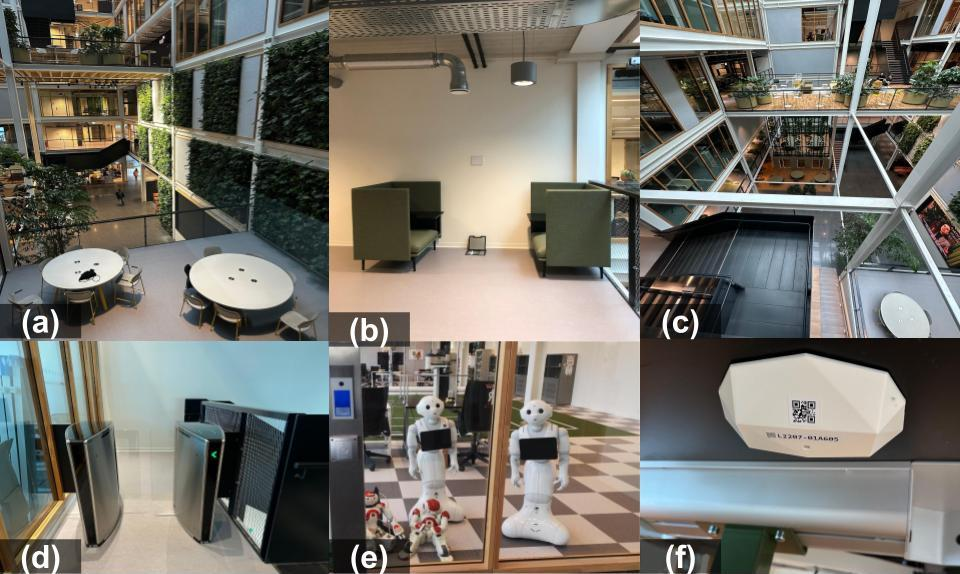
\includegraphics[width=\linewidth]{images/lab42/lab42.jpg}
    \caption{Experience-shaping elements in the smart building: (a) Open layout with plant walls in the glass atrium and group tables promoting collaboration. (b) Quiet and individual spaces with focused lighting. (c) The open central atrium surrounded by quiet outer zones. (d) Access management controlled via card readers. (e) Colourful and ``curious'' robots at the entrance. (f) Occupancy sensors under work tables to monitor and manage traffic.}
    \label{fig:lab42-examples}
    \Description{Composite photograph of the LAB42 smart building showing six elements: (a) a glass atrium with plant walls and shared tables, (b) enclosed individual workspaces with focused lighting, (c) a central open atrium surrounded by quieter outer zones, (d) card-reader access points between areas, (e) colourful robots positioned at the building entrance, and (f) occupancy sensors mounted beneath work tables.}
\end{mainfigure}


\section{Study Context: A Public Educational ``Smart'' Building}
\label{sec:ch3-lab42}

Our study was conducted in a public building in Western Europe, used by students, researchers, and industry partners\sidenote{https://lab42.uva.nl/}. It features a Building Management System (BMS) that regulates lighting, temperature, and air quality using occupancy and environmental data. Automated systems manage energy use, space allocation, and access control (\autoref{fig:lab42-examples}). The building’s spatial design offers different forms of experience: lower levels host an open atrium with plant walls and communal seating to foster social connection; inner rings use colour, light, and digital artefacts to stimulate curiosity and collaboration; and outer rings offer acoustically treated nooks for focused work. This combination of automation and affective spatial cues makes the building an ideal site for our inquiry, reflecting emerging ambitions in smart environments while revealing potential disconnects between what systems regulate and how occupants interpret, sense, and navigate space. We conducted two user studies in this building: an open-ended survey eliciting emotion-and-comfort-framed reflections across locations, and a walk-through study tracing how occupants interpret and adapt to their environment over time. Ethical approval was obtained from our institute’s review committee.

